%!TEX root = ../../thesis.tex


% discovery: ATLAS (gg, ZZ, WW) and CMS (gg, ZZ, WW, tt, bb)
% later supported by final Tevatron combination, VH->bb, 3.1$\sigma$ \cite{Tevatron:2012}
% since then, many more analyses dedicated to measure specific properties (updated with larger datasets => more significant)


\subsection{Mass measurement}
\label{sec:searches:mass}

The mass of the Higgs boson, \mH, is unpredicted by the Standard Model, and is very 
important to measure precisely. Once \mH is known, all the Higgs boson couplings, 
production cross sections and branching ratios can be calculated (see 
\Section~\ref{sec:properties}). The value of \mH is also important when assessing the 
theoretical implications of the discovery (see \Section~\ref{sec:implications}).

The \HepProcess{\PHiggs \HepTo \Pphoton\Pphoton} and \HepProcess{\PHiggs \HepTo \PZ\PZ} 
decay channels offer the best sensitivity to \mH, since they exhibit very clean 
experimental signatures and can fully reconstruct the Higgs boson four-momentum.
Combining these two channels gives an \mH measurement of 
\unit{\statsyst{125.5}{0.2}{0.6}{}}{\GeV} in ATLAS \cite{ATLAS:combination:2013} and 
\unit{\statsyst{125.7}{0.3}{0.3}{}}{\GeV} in CMS \cite{CMS:mass}. These results are very 
consistent, although some tension exists between the two ATLAS channels.

Nature has been kind in providing a Higgs boson with \unit{$\mH \approx 126$}{\GeV}, since 
many different production modes and decay channels should be experimentally accessible at 
the LHC (see Figures~\ref{fig:higgs_xs} and \ref{fig:higgs_br}). In particular, couplings 
to bosons and fermions can be measured, providing evidence of the two types of mass 
generation that the Higgs field is responsible for in the Standard Model.

% \begin{figure}[t]
% 	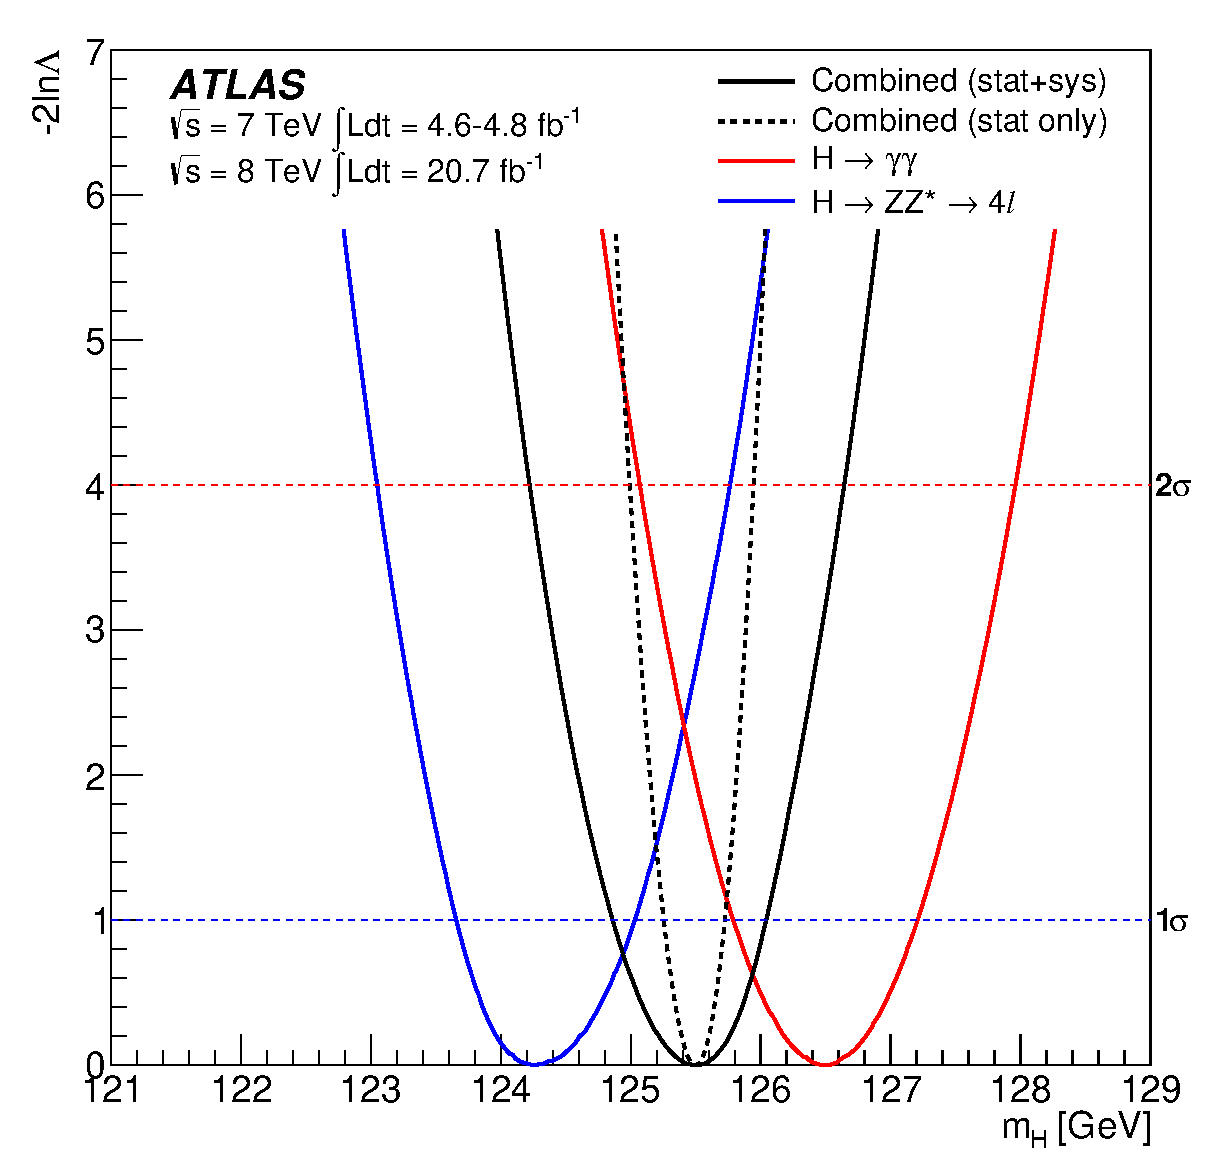
\includegraphics[width=0.48\textwidth]{tex/conclusions/atlas_mass}
% 	\hfill
% 	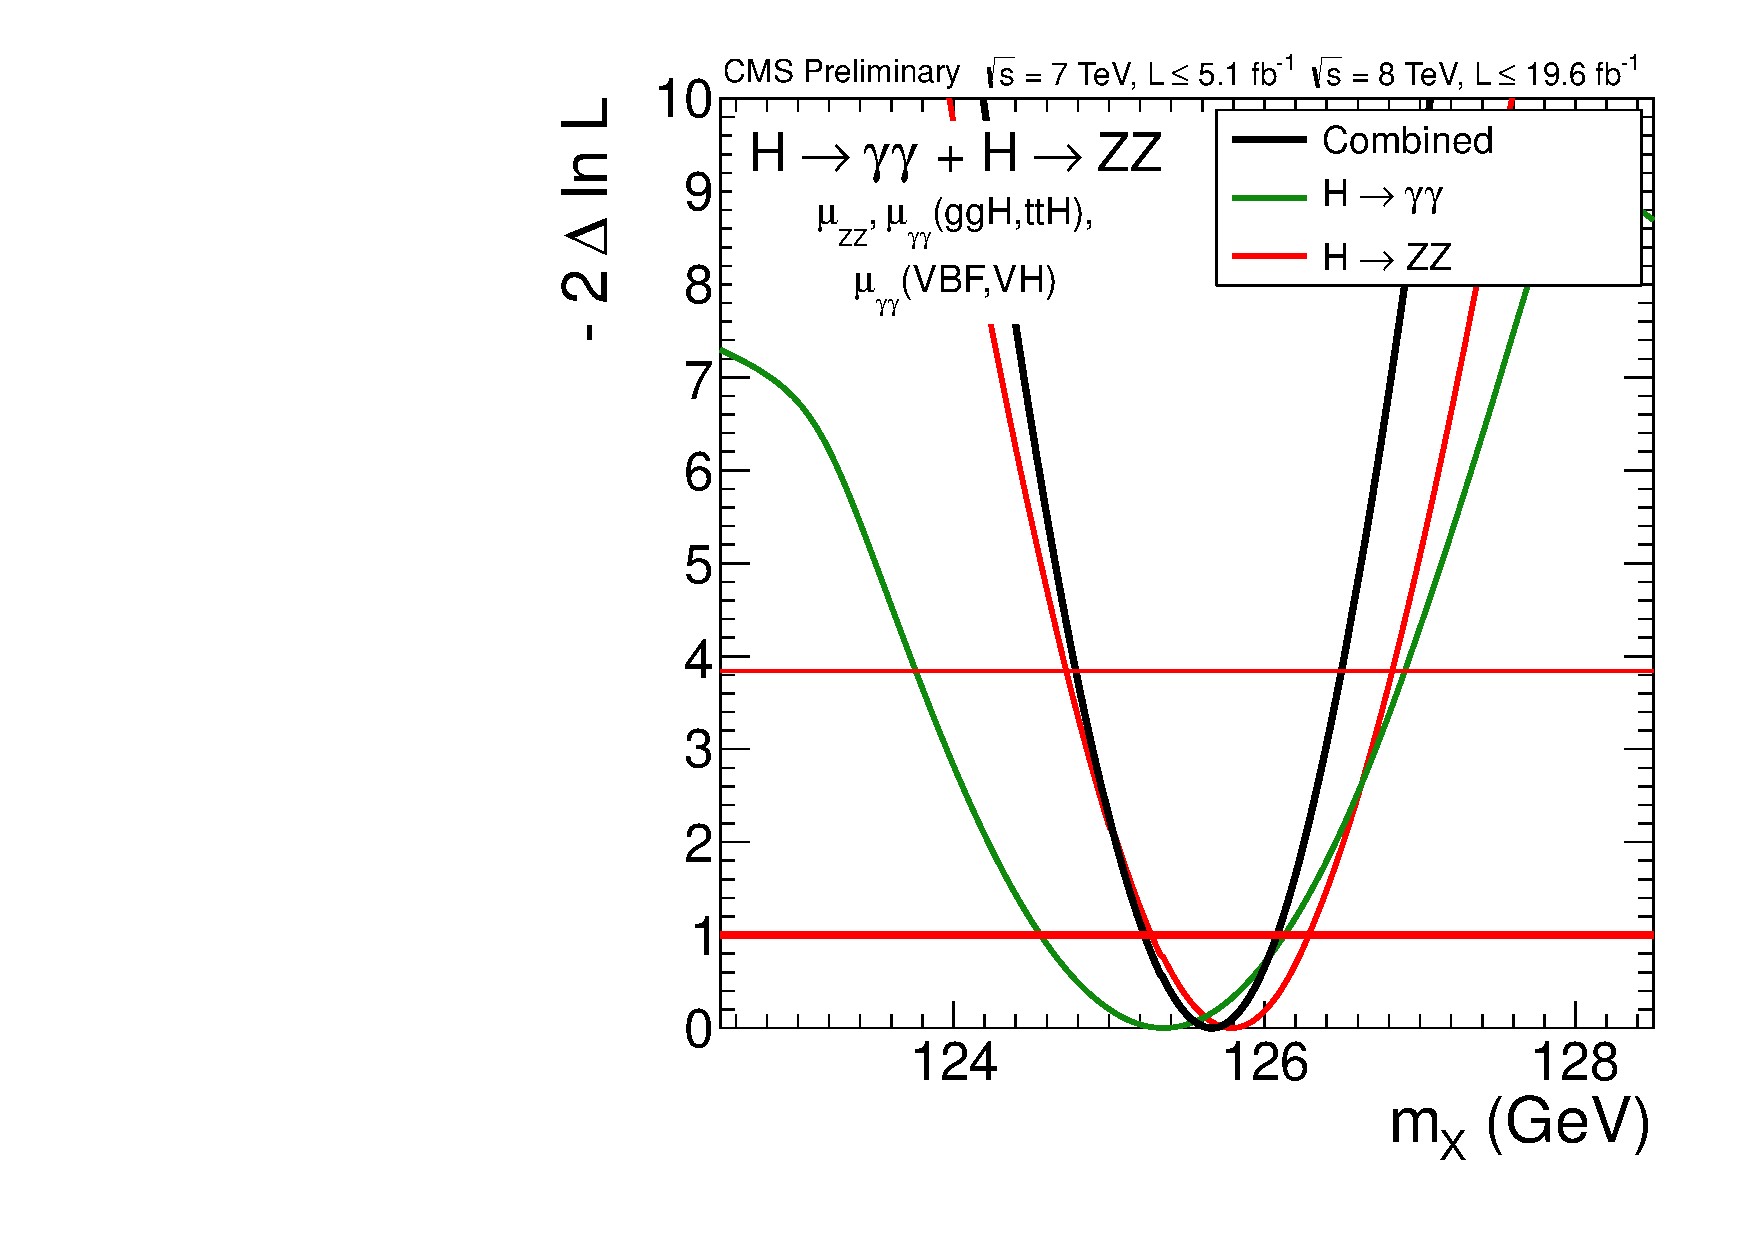
\includegraphics[width=0.49\textwidth]{tex/conclusions/cms_mass}
% 	\caption{Profile likelihood ratio test statistic as a function of \mH measured by the 
% 	ATLAS (left) and CMS (right) experiments \cite{ATLAS:combination:2013,CMS:mass}. 
% 	Measurements of \HepProcess{\PHiggs \HepTo \Pphoton\Pphoton} and \HepProcess{\PHiggs 
% 	\HepTo \PZ\PZ} and their combination are shown.}
% 	\label{fig:concl:mass}
% \end{figure}



\subsection{Coupling measurements and limits}
\label{sec:searches:couplings}


\subsection{Spin-parity measurement}
\label{sec:searches:spin}

